\section{Implementacja platformy}
\label{cha:impl}

Rozwiązanie zaprezentowane w niniejszym artykule zostało napisane w języku Java, z wykorzystaniem Ontology API biblioteki Apache Jena. Biblioteka ta pozwala na mapowanie różnego rodzaju reprezentacji ontologii na klasy Java. Do transferowania naszych danych wykorzystamy bibliotekę Apache CXF, a dokładniej jej moduł REST, który pozwoli nam na przesyłanie zserializowanych danych przez protokół HTTP.
Schema klienta został przedstawiony na Rys. \ref{fig:javaclient}

\end{multicols}
\begin{figure}[p]
	\centering
	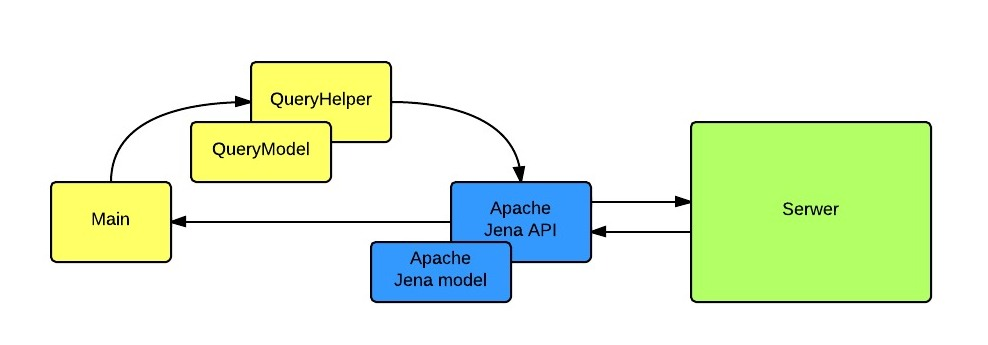
\includegraphics[scale=0.2]{pics/Scheme}
	\caption{Schemat klienta JAVA}
	\label{fig:javaclient}
\end{figure}
\begin{multicols}{2}

\subsection{Reprezentacja danych}
\label{sec:persist}

Ontology API biblioteki Apache Jena pozwala między innymi na budowanie oraz importowanie modeli ontologii. Stworzenie nowego modelu ontologii oraz zaimportowanie do niego już istniejącej ontologii zapisanej w formacie OWL przedstawiono na rysunku. Przykładowy graf wygenerowany z części ontologii widoczny jest na rysunkach \ref{fig:placeont} oraz \ref{fig:roleont}

\end{multicols}
\begin{figure}[p]
	\centering
	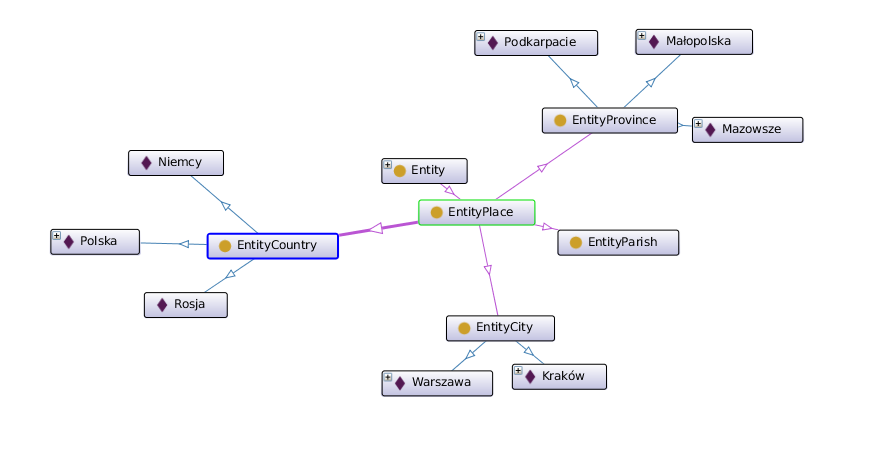
\includegraphics[width=\textwidth]{pics/EntityPlaceOntology}
	\caption{Przykład Ontologii Opartej o HL7 (EntityPlace)}
	\label{fig:placeont}
\end{figure}
\begin{figure}[p]
	\centering
	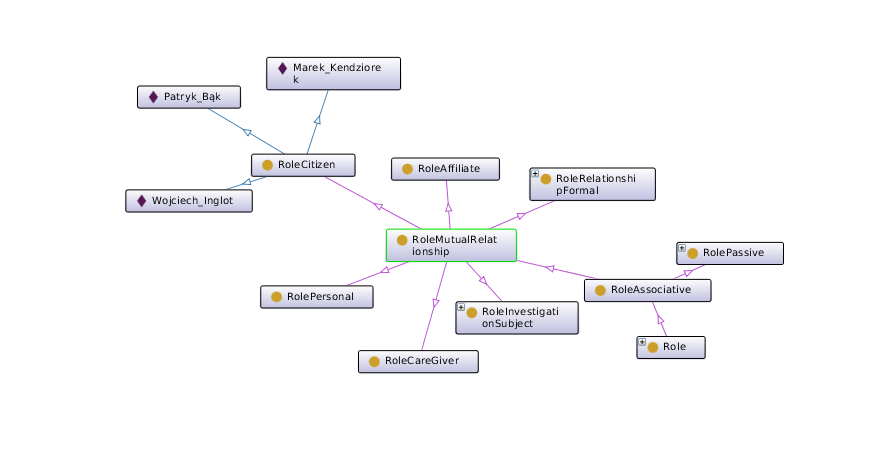
\includegraphics[width=\textwidth]{pics/RoleOntology}
	\caption{Przykład Ontologii Opartej o HL7 (Role)}
	\label{fig:roleont}
\end{figure}
\begin{multicols}{2}

\subsection{Transfer danych}
\label{sec:transfer}

W projekcie uruchomiony został serwer HTTP Fuseki. Pozwala on na przechowywanie i udostepnienie danych wczytanych z plikow OWL poprzez zapytania HTTP. W jego wewnętrznej bazie danych budowane są grafu do których aplikacje klienckie odwołują się w zapytania SPARQL.

\subsubsection{Instalacja}

~Instalacja Jeny i Fuseki ogranicza się do dodania do zmiennych środowiskowych ścieżek do paczek.
\begin{lstlisting}
export JENA= /Users/XXXX/Fuseki/apache -jena-2.11.0/
export FUSEKI= /Users/XXXX/Fuseki/jena -fuseki-1.0.0/
\end{lstlisting}

\subsubsection{Uruchomienie serwera}

~Standardowo serwer FUSEKI uruchamiany jest pod wirtualną domeną \quotedblbase localhost\textquotedblright i na porcie 3030.

Uruchomienie serwera FUSEKI:
\begin{lstlisting}
./fuseki-server --update --loc=/Users/~/MyTDB/ /ds &
\end{lstlisting}

\subsubsection{Załadowanie pliku z ontologią}

~Załadowania pliku OWL (poprzez konsolową komendę):

\begin{lstlisting}
./s-put http://localhost:3030/ds/data default /Users/XXXX/RIMV3OWL.owl
\end{lstlisting}

\subsubsection{Tworzenie zapytania SPARQL}

~Wysłanie zapytania SPARQL wypisującego \quotedblbase koncepty\textquotedblright z załadowanego grafu:

\begin{enumerate}
\item Tworzenie zapytania.
\begin{lstlisting}
select distinct ?Concept where {[] a ?Concept}
\end{lstlisting}
\item Tworzenie zapytania HTTP POST, gdzie:
\begin{itemize}
\item jako URI podajemy sufix prowadzący do punktu końcowego (eng. endpoint) i doklajemy końcówkę /query
\item w parametrze POST/GET \quotedblbase query\textquotedblright podajemy stworzone zapytanie 
\item opcjonalne parametry: output (np. \quotedblbase json\textquotedblright ), default-graph-uri
\end{itemize}
\item W efekcie otrzymujemy zapytanie (dla punktu końcowego \quotedblbase ds\textquotedblright :
\end{enumerate}
